%TABLES, MULTIROW, MULTICOLUMN   
\documentclass[24pt, a4paper]{article} % pt indicates the font size of the prepared document
\usepackage[utf8]{inputenc} %indicates the encoding of the document
\usepackage{multicol}
\usepackage{graphicx}
\usepackage{multirow}
\usepackage{cite}
\usepackage{amsmath,amssymb,amsfonts}
\usepackage{algorithmic}
\usepackage{graphicx}
\usepackage{textcomp}
\usepackage{xcolor}
\usepackage{minted}
\usepackage{hyperref}
\usepackage{soul}
\usepackage{float}
\usepackage[margin=1.0in]{geometry}

\title{Wireless Mobile Network Simulation Assignment Report}
\author{Md. Asif Haider \\ 
ID: 1805112}

\date{\today}

\begin{document}

\maketitle
\pagebreak %This will force the rest of the document to start in another page.

\tableofcontents
\pagebreak

\section{Specification}
\label{sec:intro} %This will be used while referencing this section
In this assignment, we were asked to perform some wireless mobile network simulations using Network Simulator v2 (NS2) software. As specified for student ID 1805112, the set of network stack components and global simulation parameters are as follows:

\begin{itemize}
    \item \textbf{Wireless MAC Type:} Wireless 802.11 protocol
    \item \textbf{Routing Protocol:} AODV
    \item \textbf{Agent:} UDP
    \item \textbf{Application:} CBR traffic 
    \item \textbf{Node Positioning:} Random
    \item \textbf{Flow Type:} 1 Source, Random Sink (except source itself)
    \item \textbf{Interface Queue:} Droptail, Priority Queue, Maximum size 50 packets
    \item \textbf{Antenna:} Omni-directional, unity gain
    \item \textbf{Radio Propagation Model:} Two ray ground
    \item \textbf{Node Speed:} Randomly between 1 m/s and 5 m/s
\end{itemize}
We also defined the data link layer and the wireless shared media interface with default values provided by the simulator.

\section{Description}
\subsection{802.11 MAC Protocol}

IEEE 802.11 is a set of \textbf{Physical and Data Link layer} standards for \textbf{W}ireless \textbf{L}ocal \textbf{A}rea \textbf{N}etwork \textbf{(WLAN)} communication. It is commonly used to provide wireless connectivity in homes, offices, and public spaces. There are several different versions of 802.11 providing different levels of performance and security. \\


These networks can be used in two modes. The \textbf{Infrastructure} mode consists of client devices associated with an \textbf{Access point (AP)}, which in turn, is connected with other networks. The clients send and receive data packets via the AP. \\

The other mode is known as the \textbf{Ad Hoc} network, which is a collection of computers associated with each other to directly send and receive frames. There is no separate access point here. We are concerned with this ad hoc type of network in this simulation. 

\subsection{AODV Routing Protocol}

Network of nodes staying near each other are known as \textbf{M}obile \textbf{A}d hoc \textbf{Net}works \textbf{(MANETs)}. As opposed to wired networks, the topology in ad hoc networks might be changing all the time, making routing in these networks more challenging. We used MANET for this simulation. \\

\textbf{A}d hoc \textbf{O}n-demand \textbf{D}istance \textbf{V}ector \textbf{(AODV)} is one of the most popular routing protocols used for MANETs in \textbf{Network layer}. At each node, AODV maintains a routing table. The routing table entry for a destination contains three essential fields: a next hop node, a sequence number, and a hop count. All packets destined for the destination are sent to the next hop node. The sequence number acts as a form of time-stamping. The hop count represents the current distance to the destination node. \\

In AODV, routes to a destination are discovered only when a source wants to send a packet to that particular destination, eventually saving much of the wasted work needed when the topology changes before that route is used. This property of discovering routes exactly when they are needed is what makes this hop-by-hop routing algorithm \textbf{on demand}. This is achieved by a request-response cycle based on RREQ and RREP messages between the nodes. 

\subsection{UDP Agent}

The \textbf{U}ser \textbf{D}atagram \textbf{P}rotocol \textbf{(UDP)} agent is a type of network agent that uses the \textbf{Transport layer} UDP protocol to send and receive data. UDP is connectionless, meaning it does not establish a dedicated connection before sending data. Instead, it sends packets of data called datagrams to the destination without establishing a connection (like a virtual circuit) beforehand. It uses a small packet size with a small header (8 bytes). This fewer bytes in the overhead makes UDP protocol need less time in processing the packet and need less memory.\\

UDP is a good choice for applications that need to send a large amount of data quickly, such as streaming media or online gaming. Using UDP is faster as integrity is checked at the arrival time using checksum. However, it does not guarantee delivery. In contrast with TCP, no acknowledgment is issued here. It does not do flow control, congestion control, or even re-transmission upon receipt of a bad/corrupted packet. Hence, it may not be the best choice for applications requiring reliable data transfer.

\subsection{CBR Traffic}

\textbf{C}onstant \textbf{B}it \textbf{R}ate \textbf{(CBR)}, in general, is a term used in telecommunication relating to the quality of service. It also refers to a type of network traffic generator in \textbf{Application layer}. CBR is a term describing the behavior of a traffic agent (usually UDP), that generates bits at a constant specified rate with low latency. It is mainly used in real-time streaming applications so that the content can be transferred through a limited channel capacity. 

\section{Result and Discussion}

With our personalized specific parameters and global parameters fixed, we were asked to vary the following baseline parameters below:

\begin{itemize}
    \item Area Size: 500m x 500m
    \item Number of Nodes: 40
    \item Number of Flows: 20
\end{itemize}

For each of the varying parameters, we were asked to plot 4 graphs showing the change of 4 different metrics listed below: 

\begin{itemize}
    \item Network throughput
    \item End-to-end delay
    \item Packet delivery ratio (total no. of packets delivered to end destination / total no. of packets sent)
    \item Packet drop ratio (total no. of packets dropped / total no. of packets sent)
\end{itemize}

The throughput is the measure of how fast we can actually send data through the network. It is the measurement of the number of packets that are transmitted through the network in a unit of time. It is desirable to have a network with high throughput. \\

End-to-end delay is the average time delay consumed by data packets to propagate from source to destination. This delay includes the total time of transmission i.e. propagation time, queuing time, route establishment time, etc. A network with minimum average end-to-end delay offers better speed of communication. \\

The packet delivery ratio is the ratio of the number of packets received at the destination to the number of packets generated at the source. A network should work to attain a high delivery ratio in order to have a better performance, which shows the amount of reliability offered by the network. \\

The packet drop ratio is just the complement of the delivery ratio. The lower the drop rate, the better the network stack. \\

\subsection{Area Size}

We varied area sizes among 250m x 250m, 500m x 500m, 750m x 750m, 1000m x 1000m, and 1250m x 1250m.

\begin{figure}[H]
    \centering
    \centering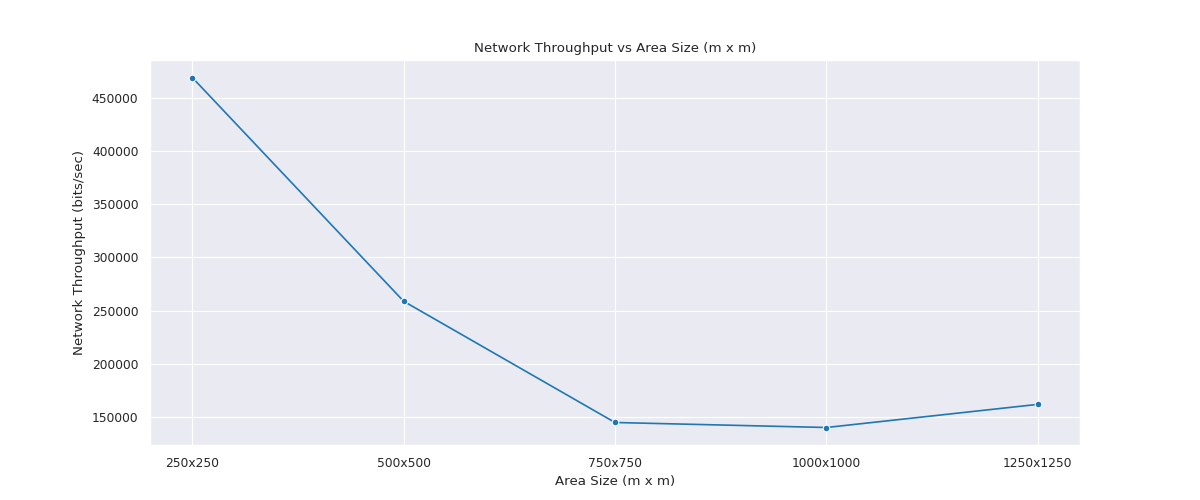
\includegraphics[width = \linewidth]{Figure_1.png}
    \label{fig:1}
\end{figure}


\begin{figure}[H]
    \centering
    \centering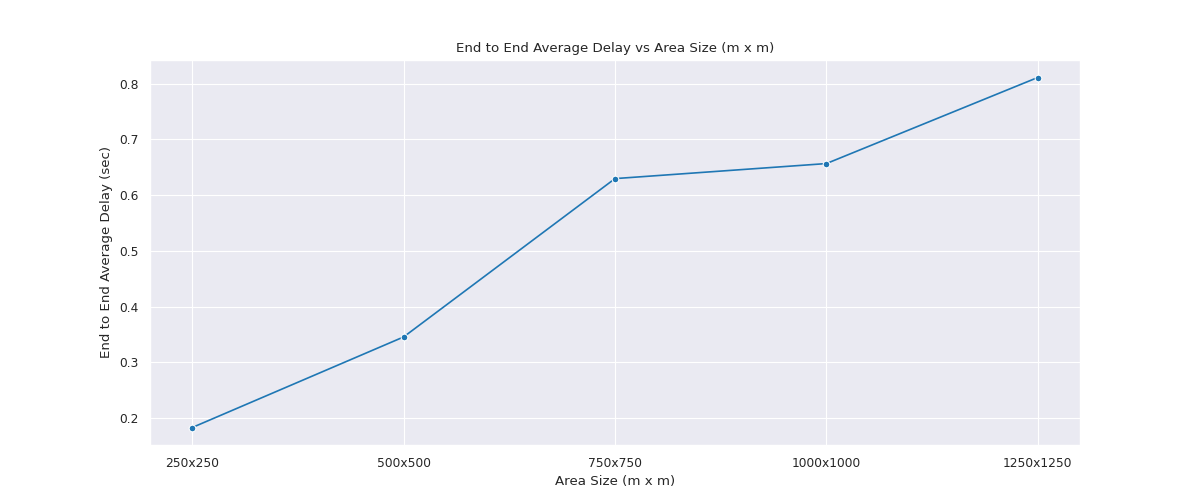
\includegraphics[width = \linewidth]{Figure_2.png}
    \label{fig:2}
\end{figure}



\begin{figure}[H]
    \centering
    \centering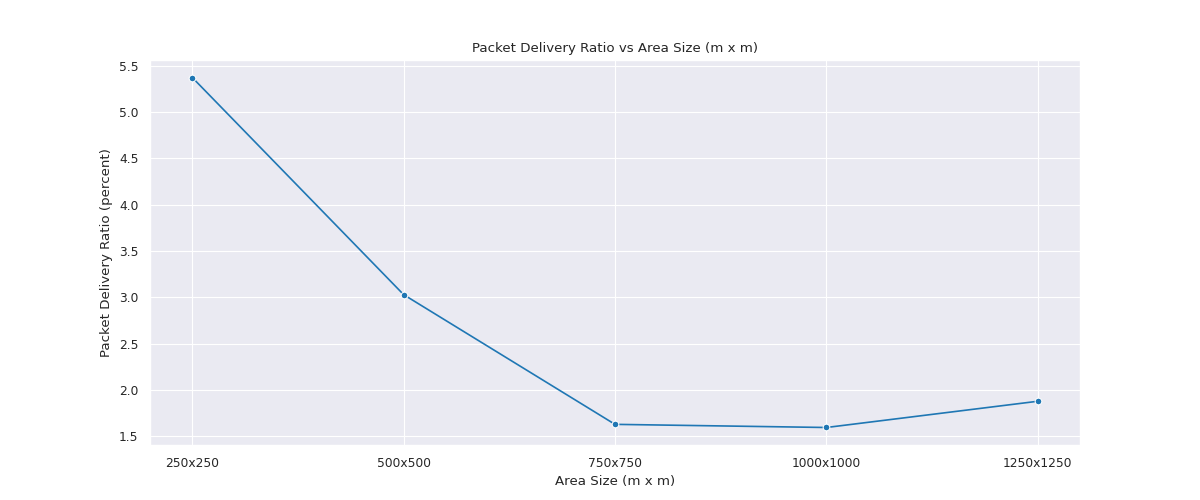
\includegraphics[width = \linewidth]{Figure_3.png}
    \label{fig:3}
\end{figure}

\begin{figure}[H]
    \centering
    \centering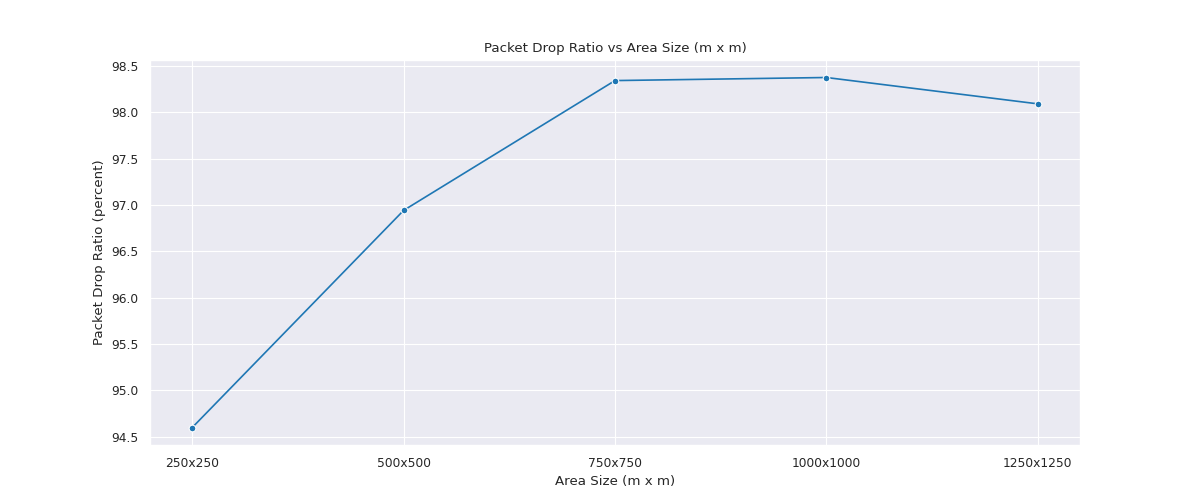
\includegraphics[width = \linewidth]{Figure_4.png}
    \label{fig:4}
\end{figure}

The efficiency of packet transmission in ad hoc networks is influenced by the physical distance between nodes. Hence, as the area size increases, the throughput decreases. Similarly, the average delay increases with the area size increment. \\

The packet delivery ratio usually decreases as the area grows larger, and the drop ratio increases for the same reason. UDP being an unreliable protocol usually leads us to a higher rate of packet loss as shown in the figures above. 

\subsection{Number of Nodes}

We experimented with various node counts among 20, 40, 60, 80, and 100.

\begin{figure}[H]
    \centering
    \centering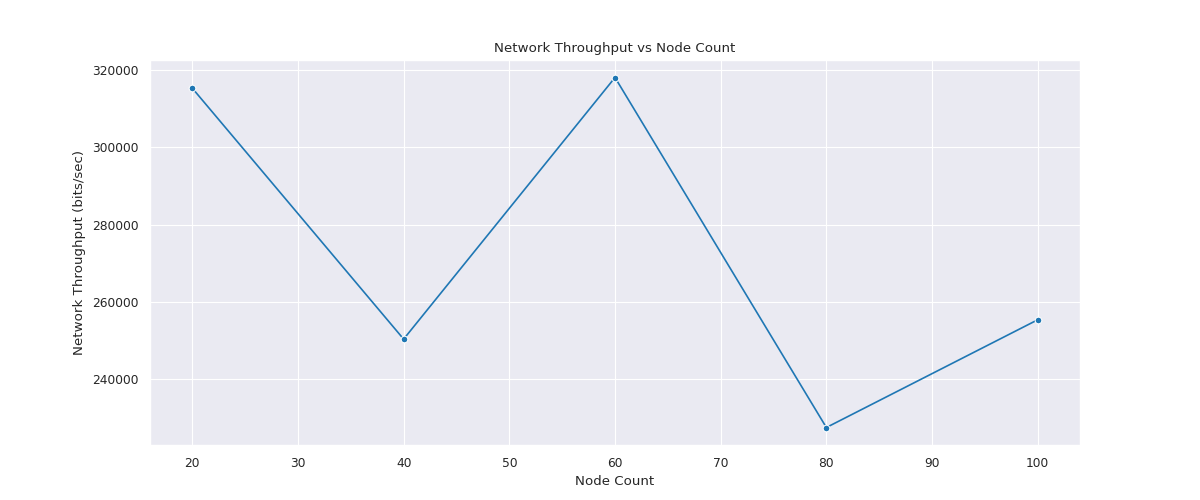
\includegraphics[width = \linewidth]{Figure_5.png}
    \label{fig:5}
\end{figure}

\begin{figure}[H]
    \centering
    \centering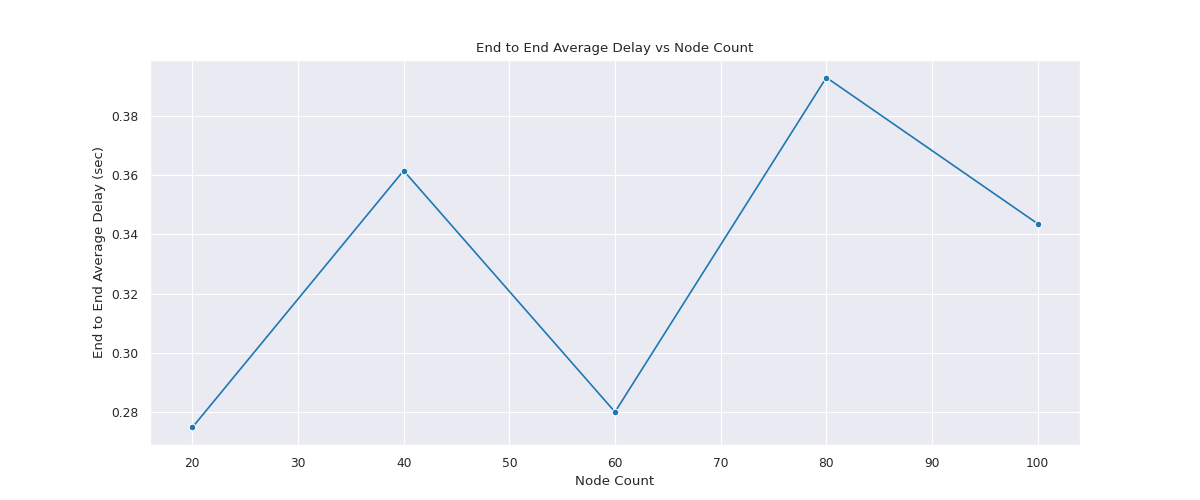
\includegraphics[width = \linewidth]{Figure_6.png}
    \label{fig:6}
\end{figure}

\begin{figure}[H]
    \centering
    \centering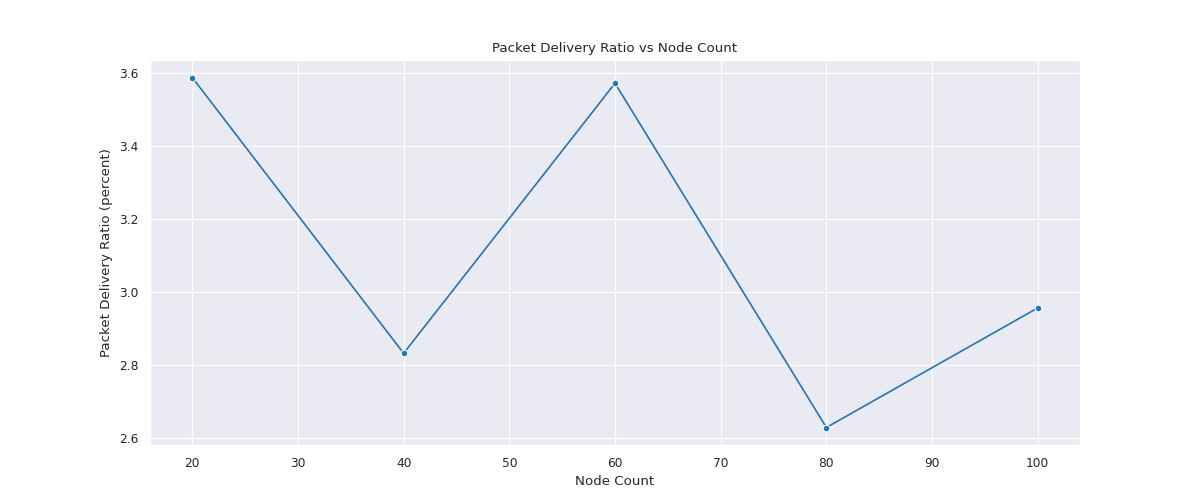
\includegraphics[width = \linewidth]{Figure_7.png}
    \label{fig:7}
\end{figure}

\begin{figure}[H]
    \centering
    \centering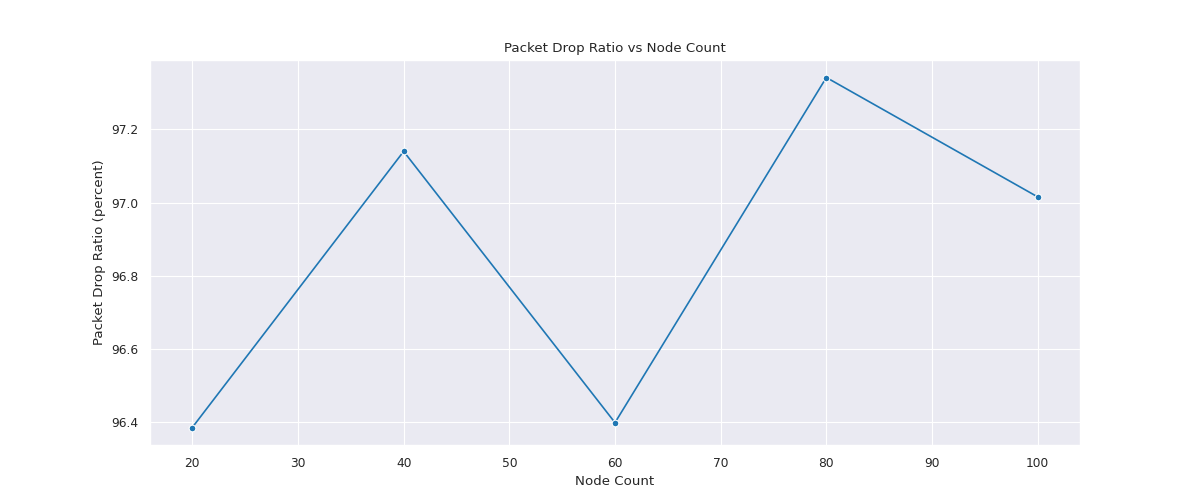
\includegraphics[width = \linewidth]{Figure_8.png}
    \label{fig:8}
\end{figure}

As can be seen from the graphs, the metrics we used are not following any particular pattern with respect to varying node count. It rather fluctuates for all four metrics. \\ 

One potential reason behind the unpredictability of packet transmission in ad hoc networks might be the random positioning and movement of nodes, effectively changing the network structure as the node count grows larger.


\subsection{Number of Flows}

We plotted various numbers of flows from 10, 20, 30, 40, and 50.

\begin{figure}[H]
    \centering
    \centering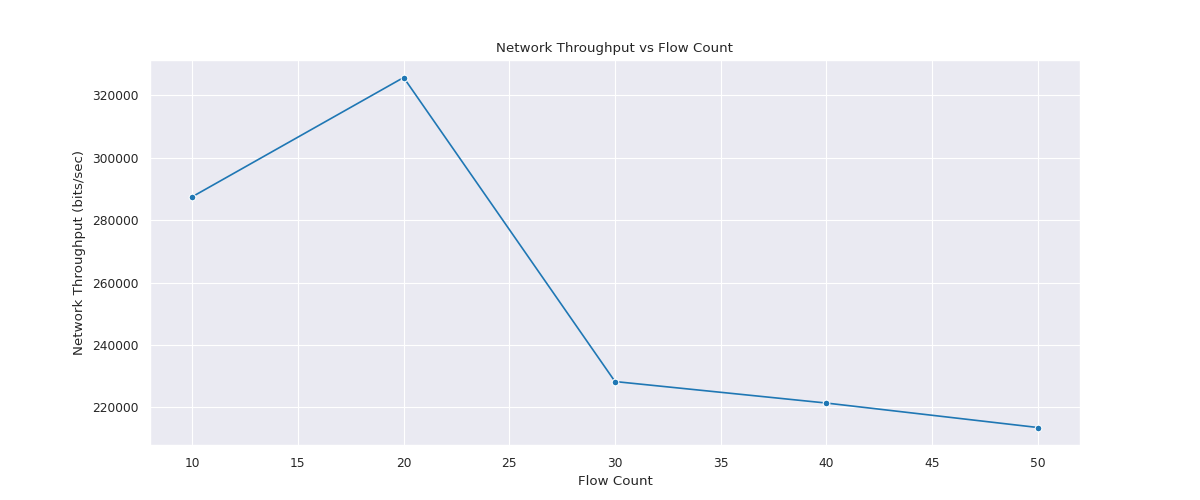
\includegraphics[width = \linewidth]{Figure_9.png}
    \label{fig:9}
\end{figure}

\begin{figure}[H]
    \centering
    \centering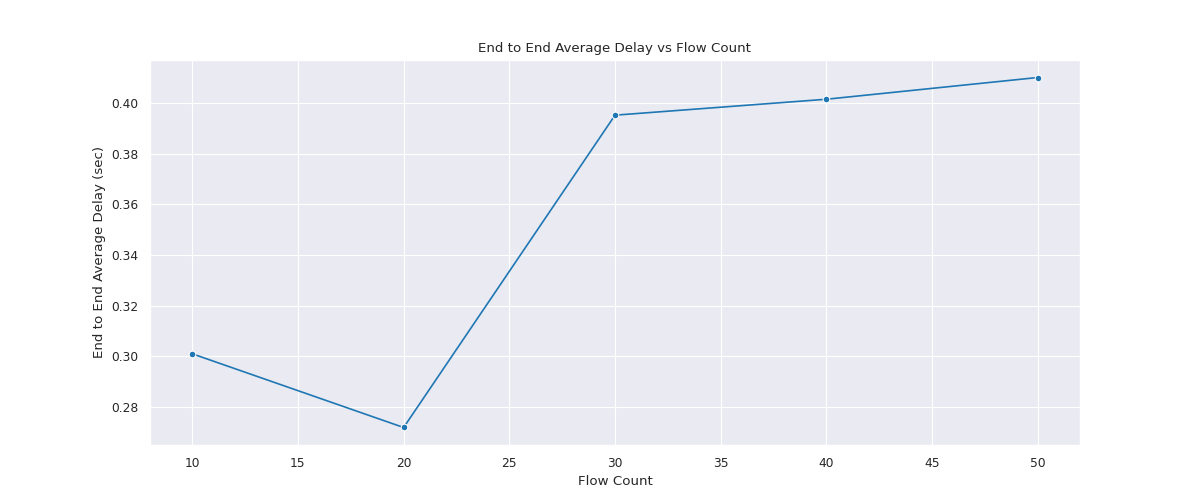
\includegraphics[width = \linewidth]{Figure_10.png}
    \label{fig:10}
\end{figure}

\begin{figure}[H]
    \centering
    \centering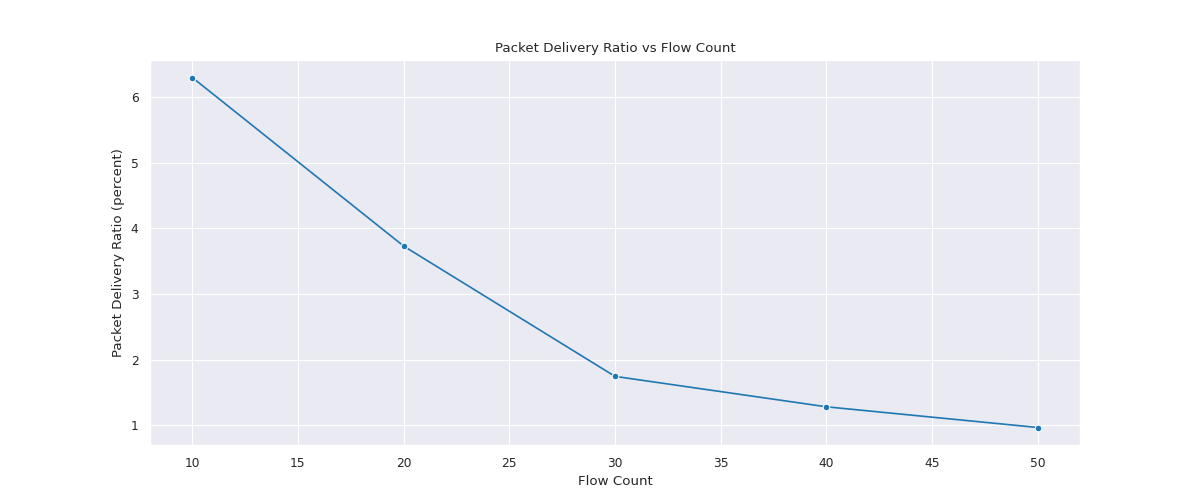
\includegraphics[width = \linewidth]{Figure_11.png}
    \label{fig:11}
\end{figure}

\begin{figure}[H]
    \centering
    \centering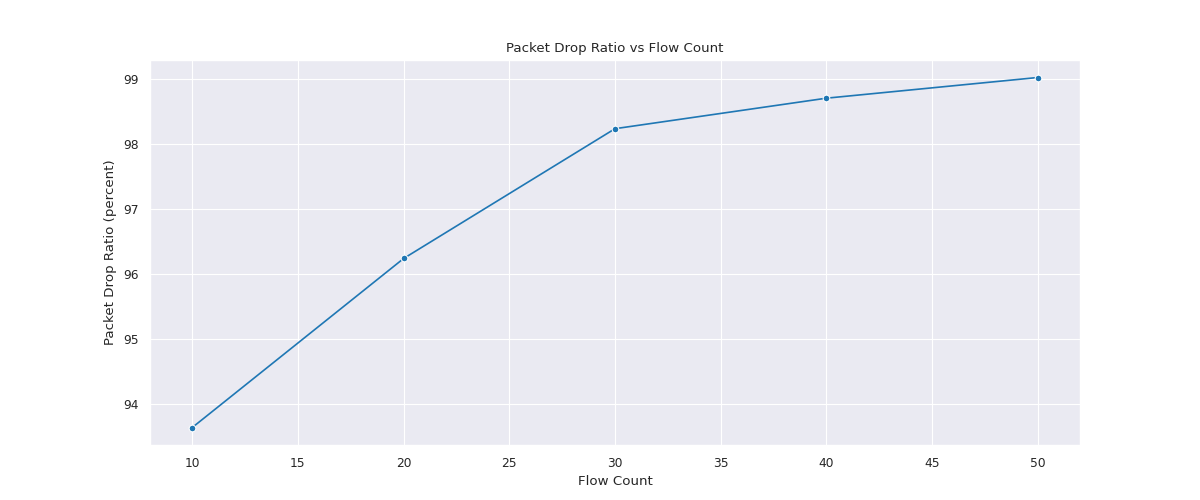
\includegraphics[width = \linewidth]{Figure_12.png}
    \label{fig:12}
\end{figure}

In this experiment of varying the flow count, the packet delivery and drop ratios follow a certain pattern as expected. The volume of concurrent data flows increases as we increment the flow count, possibly resulting in a drop in the delivery ratio. \\

The shapes of the throughput and delay graph again show a variety from a little to a significant amount, as the sink nodes are created randomly by our simulator setup.

\end{document}